%---------------------------------------------------------------------------------------------------
%		elasticity.tex
%
%	This is the main file of the chapter that talk about elasticity.
%
%	Author: Andrea Meneghinello
% Version: 0.1
%	Table of changes:
%		17/03/2016 -> document definition
%---------------------------------------------------------------------------------------------------
\section{Introduction}
\label{sec:elasticity-introduction}
A requirement for distributed services is availability: they must remain regularly available to be
used by as many customers as needed with \keyword{acceptable performance} and \keyword{scalability}.
Distributed services and systems have always been required to be scalable. Replication of services
components, in order to balance the workload arriving to each replica, has been the chosen approach.

Services needed to be carefully designed in order to minimize synchronization needs among their
components with the aim of not blocking their execution. Evidently, unlimited scalability could not be
achieved since it requires infinite infrastructure resources. So, traditionally, scalability of a
service depends on its software architecture being limited by the amount of hardware resources secured
in the data-centre where it was deployed.

As we have seen in the previous chapter, the advent of cloud computing partially broke those limits, but
elasticity management remains not trivial.

According to the \ac{nist} definition (given in Section
\ref{sec:background-cloudComputing-cloudServiceModels}), \ac{paas} gives freedom to the customer regarding
application reconfiguration, since end-users should only deal with the general ``configuration settings
for the application-hosting environment'' but do not need to worry about the mechanism being needed
for implementing those reconfigurations. Reconfiguration management is the responsibility of \ac{paas}
providers. Since every cloud service should be elastic (accordingly with cloud definition), this mean
that \ac{paas} providers should deal with many mechanism that automate the service scalability and
adaptability.

However, the level of automation needed to approach a cost-optimal exploitation of the service is still
changing nowadays because of the many aspects that should be considered. On one hand, scalability
decisions must match what has been stated in the \ac{sla}. This means that those decisions should be
taken as soon as the workload or the service performance starts to vary, which strongly suggests the
need to include some workload prediction mechanism. Nevertheless, forecasting techniques are not perfect
hence, they should be complemented with other reactive mechanism; e.g. when the resulting service
performance level do not comply with what is being specified in the \ac{sla} or lead unnecessary
over-provisioning costs, service providers should take appropriate actions. Those actions may consist
in adding service instances or migrating those instances to better \ac{vm}s when service capacity
should be increased, or in the opposite case, in releasing instances when service capacity need to be
decreased.

One of the regular dimensions in \ac{sla}s is availability. Successful distributed services are
concurrently used by many customers. Service providers should guarantee service continuity, otherwise
service clients will not rely on that provider and they will look for another, more reliable, one.
Unfortunately, since complex software systems are always in need of modification, both platform and
service components need to be eventually updated in order to fix bugs, remove security vulnerabilities
or enhance their functionality. This software upgrading process might endanger the availability levels
specified in a \ac{sla}. So, this is another source of trouble for service providers.

\subsection{Requirements}
\label{sec:elasticity-requirements}
\citeauthor{herbst2013elasticity} in \cite{herbst2013elasticity} defines elasticity in cloud computing
model as:

\begin{quote}
	``the degree to which a system is able to adapt to workload changes by provisioning and
	deprovisioning resources in an automatic manner, such that at each point in time the available resources
	match the current demand as closely as possible.''
\end{quote}

The given definition states that elasticity is basically the combination of two complementary
dimensions: \keyword{scalability} and \keyword{adaptivity}. Therefore elastic services (or applications)
should be able to collect new computing resources when their workload is increased, but also to discard
any exceeding resources when such workload decreases. Additionally, such resource management should be
the most autonomous as possible; e.g. driven by the system itself without any human operator or
administrator interference.

From \citeauthor{herbst2013elasticity} definition of elasticity, some requirements may be
identified: \keyword{autonomy}, \keyword{scalability} and \keyword{adaptability}.

Those are general requirements that have to be considered in any kind of elastic service or application,
but we are interested on the \ac{paas} cloud computing service model so other requirements arise;
they are: \keyword{\ac{sla}-awareness}, \keyword{composability} and finally \keyword{service continutiy
in software upgrades}.

In the following sections we will cover in deep all these requirements giving its definition and
some explanations for each one.

\subsubsection*{Autonomy}
\label{sec:elasticity-requirements-autonomy}
Platforms being provided in \ac{paas} service model should deal itself (ideally without any human
interaction) with the elastic behaviour of the services deployed by its customers.

In order to have an autonomic behaviour, an application or service should be carefully designed. In 
\cite{ibm2005architectural} a system is considered autonomic when it is able to self-manage with a
minimum of human interference. In that case, such software elements should be self-configuring,
self-healing, self-optimising and finally self-protecting. To this end, a set of autonomic software
components should be controlled by an autonomic manager, which is governed by a major-loop
composed by four different stages:

\begin{enumerate}
	\item{\keyword{monitor}: in this stage some information is collected by sensors on each managed
		element. These data are then filtered and aggregated in order to build a coherent response. The
		data being considered consist of multiple metrics ad descriptions of the current resource
		topology;}
	\item{\keyword{analyse}: the data coming from the previous stage are correlated in order to consider
		some behavioural models; this allows the autonomic manager to learn from the environment and helps
		to predict future situations for the managed elements;}
	\item{\keyword{plan}: considers the information provided by the previous stage, and decides the
		actions to be performed in order to reach the system goals, according to existing policies;}
	\item{\keyword{execute}: finally autonomic manager applies those actions to the managed elements
		though the corresponding effectors.}
\end{enumerate}

Each stage is continuously being applied and its output is considered by the next step in the control
loop. To this end, the stages may access to a shared \keyword{knowledge base} where global policies
can be found and interesting information can be generated in each stage. In most cases, such data
needs to be considered in the first two stages.

This general picture of autonomic computing can be easily tailored for cloud computing systems that
follows the \ac{paas} service model. Through autonomic manager we want to reach a combination of:

\begin{itemize}
	\item{a general economic goal on which we want to minimize the cost of the underlying infrastructure,
		which is required to support all the software deployed on the platform; and}
	\item{a specific set of rules, that depends on each customer applications deployed (\ac{sla}).}
\end{itemize}

\subsubsection*{Scalability}
\label{sec:elasticity-requirements-scalability}
In order to have an elastic system the software services it provides should be \keyword{scalable}. This
means that when incoming workload is increased, the capacity of the serving nodes should be also
enlarged. There are different scalability systems: \keyword{replication}, \keyword{redemensioning} and
finally \keyword{migration}.

Replication or scaling horizontally means adding (or removing) nodes in a system, for executing additional
server instances when such serving capacity needs to be increased (or decreased). This may be implemented
adding new \ac{vm}s to the current set, deploying there some instances of the required service components.
Replication is a mechanism used also to achieve service availability. Two classical replication models
exists: \keyword{active-replication} on which every client request is forwarded to all the server replicas,
and every one executes directly each requests; and \keyword{passive-replication} on which every client request
is sent to a special replica that serves each request and forwards any state updates to the remaining replicas.
Replication was already used before cloud computing became available. In many cases applications have adopted
low-cost commodity systems to execute tasks that once required supercomputer, because computer prices have
dropped and performance continues to increase. In addiction the development of high-performance networks,
such as Gigabit Ethernet, powered this scalability model. In this model we refer with the term
\keyword{scale-out} when we are adding new nodes in the cluster, instead with \keyword{scale-in} the opposite
scenario (when nodes are removed).

Redemensioning or scaling vertically means adding (or removing) resources to a single node in the system,
typically involving the addition (or removal) of \acs{cpu}s, memory or network capabilities. Unfortunately,
many \ac{iaas} providers do not allow \ac{vm} redimensioning at run-time. Note that this procedure requires
that either the host has free resources at redimensioning time or the other guest \ac{vm}s should also adapt
their provisioned set of resources to accommodate such redimensioning. Instead of those dynamic redimensioning
actions, most \ac{iaas} providers facilitate a static set of \ac{vm} types and the consumer is compelled 
to select which kind of \ac{vm} should be used in each image allocation. In this model we refer with the term
\keyword{scale-up} when we are adding new resources to a node, instead with term \keyword{scale-down} the
opposite scenario.

\begin{figure}
	\centering{}
	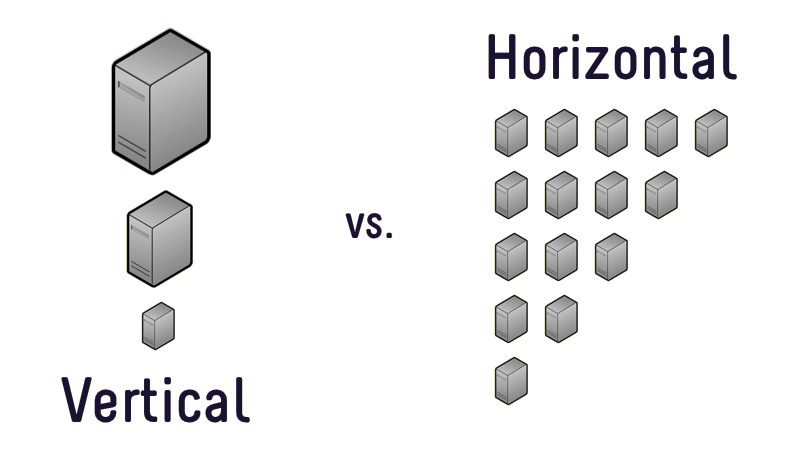
\includegraphics[width=0.6\textwidth]{chapters/elasticity/images/horizontal-vs-vertical-scaling.png}
	\caption[Difference between horizontal and vertical scalability]{The image shows the difference between
		horizontal and vertical scalability. Reading it in a bottom-up way we have respectively scale scale-up
		and scale-out. Instead, reading it in a top-down way we have respectively scale-down and scale-in.}
	\label{img:solutionSpace-elasticity-availableTypes}
\end{figure}

When the underlying infrastructure does not allow \ac{vm} redimensioning, vertical scalability may be
implemented migrating the server instances from their current \ac{vm} to another more powerful one in a 
different host. Depending on the size of the instance image, the network bandwidth and the location of
the host computers, migration may need a long time to be concluded (several seconds). Migration is a
three step procedure:

\begin{itemize}
	\item{the current instance image should be stopped. Such stop action should be initiated when such
		instance is not serving any request (e.g. when it remains in idle waiting for a new request);}
	\item{its image should be transferred to the new location;}
	\item{its activity should be restarted in the new location\footnote{If the instance identity and
		network should be preserved, some routing reconfiguration will be needed in this step.}.}
\end{itemize}

However, using \ac{paas} cloud model as a base to build our services or applications leads us to consider
only the horizontal scalability type since we are not able to manifest our preferences in term of hardware
that must be available under our services or applications. Hence our purpose in the remaining part of the
thesis is finding an application design model that is able to take advantage of the elasticity
provided by the cloud.

\subsubsection*{Adaptability}
\label{sec:elasticity-requirements-adaptability}
In elasticity we refer to adaptivity as the possibility to ``optimally'' adjusting the computing capacity
of a given service to the current workload, at run-time. So, besides being scalable, an elastic service
should also be adjustable to the workload being received at each moment.

Adaptability as two different dimensions:

\begin{enumerate}
	\item{\keyword{adaptability}: it refers to the potential for adapting a system. This means that the
		system components have been designed considering that sooner or later they will need to be
		reconfigured or restructured in some way. It is a static dimension. An elastic system should be
		both scalable and adapting, focusing that adaptability on the tools needed for guaranteeing the
		scalability \ac{qos};}
	\item{\keyword{adaptivity}: it is the system's ability to adapt itself. An adaptive system is able
		to find out when adapting actions should be applied. This means that adaptable system becomes
		adaptive when it is able to provide an autonomous management. Since autonomy is one of the
		elasticity requirements, elastic systems need to be adaptive. To this end, their architecture
		should include monitoring, analysis, planning and execution subsystems that automate all
		reconfiguration-related decisions.}
\end{enumerate}

The are two main approaches for reaching adaptivity: \keyword{proactive} and \keyword{reactive}.

In the proactive (or predictive) case, some workload analysis or workload modelling is done in order
to predict the workload levels in the near future. With this knowledge the actions needed to correctly
adapt the service capacity to current workload are taken before hand. Hence, \ac{qos} can be easily
guaranteed when those predictions have an acceptable level of accuracy.

On the other hand, with a reactive approach, both the workload and the service behaviour are completely
monitored and adequate thresholds are set on different metrics. When those thresholds are reached some
adapting actions are started.

In conclusion, proactive systems predict the forthcoming workload and apply any need reconfigurations
before hand. Instead, reactive systems monitor the current real workload and reconfigure themselves
when that current workload reaches a level that compromises their \ac{qos}.

\subsubsection*{\acs{sla}-awareness}
\label{sec:elasticity-requirements-slaAwareness}
Cloud providers following any service model (including \ac{paas}) define a special kind of adaptive
system with autonomic behaviour, since the customer-provider relation is driven by a \ac{sla}.
\ac{sla}s partially set the goals to be achieved by a provider regarding service quality. The other
goals are related to its ``\ac{qobiz}''; i.e., those other goals deal with reducing service provisioning
costs in order to maximize the business benefit.

This induces a first differential factor between general autonomic computing systems and cloud computing
environments. All non-functions quality aspects might be included in a \ac{sla} and such \ac{sla} 
defines the quality-related objectives for those cloud providers. Besides those \ac{slo}, a \ac{sla}
should also specify which are the penalties applied to a provider when those \ac{slo}s are not achieved
(assuming that clients satisfies its part of deal).

In the (ideal) \ac{paas} service model, cloud provider should manage \ac{sla}s with a rich set of objectives.
Thus \ac{paas} customers can select the most appropriate one for deploying and managing their applications
or services. The \ac{paas} service provider with the best relation between: available resource,
application-level performance guarantees and renting costs.

So, one of the existing challenges for \ac{paas} providers is to elastically manage the services being
deployed by multiple customers providing and guaranteeing a rich set of \ac{slo}s in their \ac{sla}s.

\subsubsection*{Composability}
\label{sec:elasticity-requirements-composability}
As we argued in Section \ref{sec:elasticity-requirements-scalability}, the services being deployed in
\ac{paas} system should be automatically scaled by the \ac{paas} itself. There are multiple approaches
to achieve this.

In the first place, those services should not be monolithic; if they were the scaling decisions would
be applied to the single element that implements that service. This would mean a lack of flexibility
when we try to improve such service performance, since we could only add, remove, redimension or migrate
instances of that single kind of element. Moreover, that single element would be larger than the regular
elements of a multi-component service and this would have complicated any scaling actions to be applied
onto it.

Instead, if the service is implemented by multiple small components, their scaling action will be faster
and cheaper, since the amount of resources needed to manage them will be also smaller.